\documentclass[conference]{IEEEtran}
\usepackage{amsmath,amssymb}
\usepackage{booktabs}
\usepackage{graphicx}
\usepackage{tikz}
\usetikzlibrary{arrows.meta,positioning,fit,backgrounds,calc}
\usepackage{float}
\usepackage[hidelinks]{hyperref}
\usepackage{caption}
\captionsetup{font=small,labelfont=bf}

\title{GNN-Based BERT for Understanding Context from Music:\\
A Measured Account of Where Cross-Modal Fusion Helps and Where It Does Not}
\author{\IEEEauthorblockN{Tanvir Rahman}
\IEEEauthorblockA{Student ID 22241134\\
CSE715 --- Neural Networks, Instructor: Moin Mostakim\\
BRAC University\\
8 September 2026}}

\begin{document}
\maketitle

\begin{abstract}
\noindent
We implement the four-task GNN--BERT roadmap for music context understanding:
a BERT~\cite{bert} multi-label tag classifier, a GraphSAGE/GAT encoder over music
structure graphs, a cross-attention fusion of the two with an auxiliary
valence--arousal objective, and a contrastive dual encoder for
caption--audio retrieval. All four are trained and evaluated end to end.
Our headline finding is a correction of our own first conclusion. Under a
single learning rate, fusion does not beat its stronger unimodal branch and its
cross-attention collapses to uniform weights; with the non-BERT parameters
trained at their own rate, the same architecture beats BERT-only by $+0.075$
Macro-F1. The negative result was an optimisation artefact, and we report both
states because the diagnosis is the contribution. We show (i) that the text available for MagnaTagATune is track-level
while its clips are 29\,s segments, so $96.8\%$ of clips share an input with
another clip, capping any text-only model at Micro-F1 $0.673$; (ii) that the
official MagnaTagATune split leaks $45$ artists across train and test,
covering $61.6\%$ of test clips; (iii) that our cross-attention collapses to
exactly uniform weights (entropy $1.000$ of the uniform maximum) under a shared
learning rate, so the fusion degenerates into averaging the caption; and (iv)
that raising the learning rate of every non-BERT parameter un-collapses that attention
(entropy $0.695$, peak $4.19\times$) and lifts Macro-F1 by
$+0.067 \pm 0.023$ over five paired seeds ($p = 0.003$), the largest effect we
measured --- and one that transfers: applied to the contrastive dual encoder it
doubles retrieval R@1 and lifts R@10 from $0.0220$ to $0.0339$. A six-listener
study corroborates those retrieval numbers from the other direction (mean
$1.79/5$) and adds what recall cannot see: the ranking within the model's own
top three does not predict human judgement ($r = -0.051$).
We report every number against
an explicit baseline, including a lexical-match control that scores Micro-F1
$0.540$ where our model scores $0.565$ --- a margin small enough that, on
Macro-F1, the control actually wins.
\end{abstract}


\section{Introduction}
Musical ``context'' spans genre, mood, harmonic structure, instrumentation and
listener-facing description. Sequence models over spectrograms capture local
timbral patterns but not relational structure: how a repeated segment relates
to a chorus, or how a chord transition relates to a lyrical theme. The premise
of this project is that a graph neural network over music structure, fused with
a BERT encoder over text, should capture context that neither branch captures
alone.

We test that premise rather than assume it. Our contributions are:

\begin{itemize}\itemsep2pt
\item Complete implementations of all four tasks, with $126$ unit
tests and every result reproducible from a seeded configuration recorded
alongside it.
\item Two dataset integrity findings that change how the numbers must be read:
artist leakage in the official MagnaTagATune split, and a hard performance
ceiling induced by duplicated text inputs.
\item A quantitative diagnosis of \emph{why} our cross-attention fusion fails
to beat its text branch, using an attention-entropy measurement rather than an
inference from F1.
\item A data-scale measurement showing that our weak retrieval result is
data-limited rather than broken: R@10 grows log-linearly in paired examples
($R^2 = 0.914$) on four single-seed points, which indicates the regime rather
than a required corpus size; on that fit MusicCaps' official split is far short
of the regime the task needs.
\item Honest negative results with controls: a lexical-match baseline for
caption-based tagging, and a random-prevalence baseline for every multi-label
task --- including two conclusions of our own that we had to reverse after
correcting a checkpoint-selection error.
\end{itemize}

\section{Related Work}
\textbf{Music auto-tagging.} MagnaTagATune~\cite{mtat} with a top-50 tag vocabulary is the
long-standing benchmark for multi-label music tagging, typically approached
with convolutional networks over log-mel spectrograms. Our CNN baseline (B2)
follows that lineage. The artist-leakage problem in the conventional split has
been noted in the tagging literature; we re-measure it here rather than cite it,
and quantify its extent on our filtered subset.

\textbf{Graphs for music.} Representing a track as a graph over segments,
chords or events is motivated by the observation that musical form is
relational --- repetition, return and contrast --- and not purely sequential.
GraphSAGE~\cite{sage} and GAT~\cite{gat} are the two message-passing families named in the project
specification; we implement both. Our contribution here is negative and
practical: we show that naive cosine thresholding on raw MFCC descriptors
produces near-complete graphs, which silently reduces any GNN over them to
mean pooling.

\textbf{Cross-modal alignment.} Contrastive dual encoders trained with InfoNCE~\cite{infonce}
have become the standard recipe for aligning modalities, and MusicCaps supplies
the expert captions that make audio--text alignment feasible. Our Task 4 follows
this recipe directly, with the addition of an explicit random baseline and
gallery size on every retrieval number --- both frequently omitted, and both
necessary to interpret R@K at all.

\textbf{Multi-task emotion regression.} DEAM~\cite{deam} provides continuous
valence--arousal annotations. Because it shares no tracks with the tag corpora,
joint training requires masking rather than a single joint objective; we
implement the masked alternating-batch scheme and, unusually, report what it
costs the primary task.

\section{Method}

\begin{figure*}[t]
\centering
\resizebox{\linewidth}{!}{%
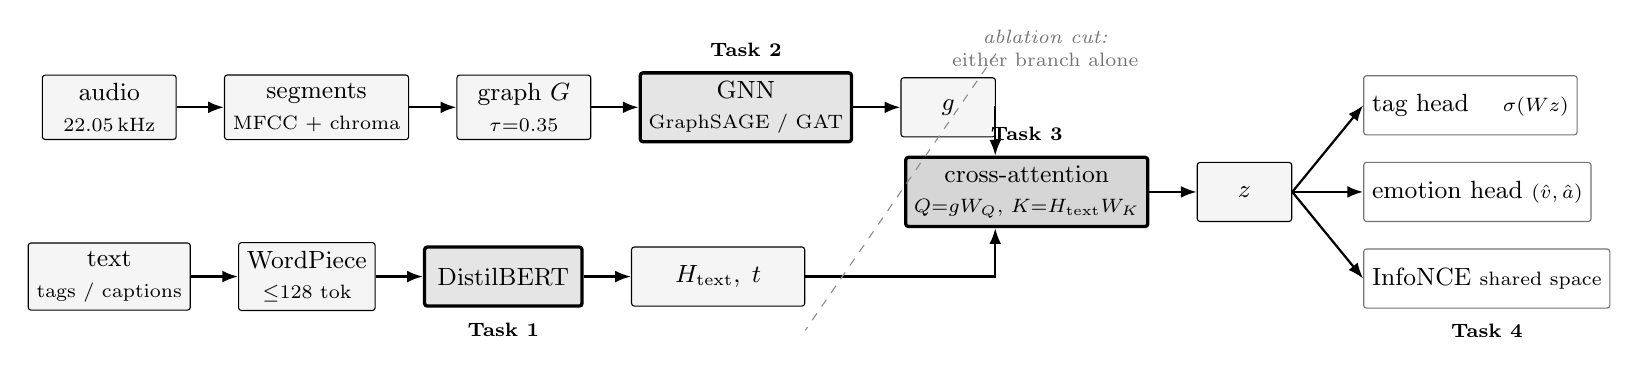
\begin{tikzpicture}[
  font=\small,
  box/.style   ={draw, rounded corners=1pt, minimum height=7.5mm, align=center, inner sep=3pt},
  data/.style  ={box, fill=black!4, minimum width=17mm},
  enc/.style   ={box, fill=black!10, minimum width=20mm, very thick},
  head/.style  ={box, fill=white, minimum width=27mm, draw=black!55},
  fuse/.style  ={box, fill=black!16, minimum width=17mm, very thick},
  ar/.style    ={-{Latex[length=2mm]}, thick},
  lbl/.style   ={font=\scriptsize, inner sep=1pt},
]
% --- audio branch ---
\node[data] (audio) {audio\\\scriptsize 22.05\,kHz};
\node[data, right=6mm of audio] (seg) {segments\\\scriptsize MFCC + chroma};
\node[data, right=6mm of seg]  (graph) {graph $G$\\\scriptsize $\tau{=}0.35$};
\node[enc,  right=6mm of graph] (gnn) {GNN\\\scriptsize GraphSAGE / GAT};
\node[box, fill=black!4, right=6mm of gnn, minimum width=12mm] (g) {$g$};

% --- text branch ---
\node[data, below=13mm of audio] (text) {text\\\scriptsize tags / captions};
\node[data, right=6mm of text, minimum width=17mm] (tok) {WordPiece\\\scriptsize $\leq$128 tok};
\node[enc,  right=6mm of tok, minimum width=20mm] (bert) {DistilBERT};
\node[box, fill=black!4, right=6mm of bert, minimum width=22mm] (h) {$H_{\text{text}},\; t$};

% --- fusion ---
\node[fuse, right=9mm of $(g)!0.5!(h)$, yshift=0mm] (fusion)
  {cross-attention\\\scriptsize $Q{=}gW_Q$, $K{=}H_{\text{text}}W_K$};
\node[box, fill=black!4, right=6mm of fusion, minimum width=12mm] (z) {$z$};

% --- heads ---
\node[head, right=9mm of z, yshift=11mm]  (tags)    {tag head \quad\scriptsize $\sigma(Wz)$};
\node[head, right=9mm of z]               (emo)     {emotion head \scriptsize $(\hat v,\hat a)$};
\node[head, right=9mm of z, yshift=-11mm] (contrast){InfoNCE \scriptsize shared space};

% --- edges ---
\draw[ar] (audio) -- (seg);  \draw[ar] (seg) -- (graph);
\draw[ar] (graph) -- (gnn);  \draw[ar] (gnn) -- (g);
\draw[ar] (text) -- (tok);   \draw[ar] (tok) -- (bert);
\draw[ar] (bert) -- (h);
\draw[ar] (g) -| ([xshift=-4mm]fusion.north);
\draw[ar] (h) -| ([xshift=-4mm]fusion.south);
\draw[ar] (fusion) -- (z);
\draw[ar] (z.east) -- (tags.west);
\draw[ar] (z.east) -- (emo.west);
\draw[ar] (z.east) -- (contrast.west);

% --- task annotations ---
\node[lbl, above=1.5mm of gnn]    {\textbf{Task 2}};
\node[lbl, below=1.5mm of bert]   {\textbf{Task 1}};
\node[lbl, above=1.5mm of fusion] {\textbf{Task 3}};
\node[lbl, right=1.5mm of contrast, rotate=-90, anchor=north] {};
\node[lbl, below=1.5mm of contrast] {\textbf{Task 4}};

% --- ablation cut lines ---
\draw[dashed, black!45] ([yshift=3mm]g.north east) -- ([yshift=-3mm]h.south east);
\node[lbl, align=center, above right=1mm and -6mm of g.north east, text=black!55]
  {\itshape ablation cut:\\ either branch alone};
\end{tikzpicture}%
}
\caption{System overview, and how the four tasks sit inside one architecture.
Audio becomes a segment graph read by the GNN into a graph vector $g$; text is
read by DistilBERT into a token sequence $H_{\text{text}}$ and its pooled vector
$t$. Task 1 is the text branch with a tag head; Task 2 is the graph branch with
a genre head; Task 3 fuses them by letting $g$ query $H_{\text{text}}$, then
feeds the tag and emotion heads; Task 4 reuses the same two encoders as
projection towers trained contrastively. The ablation table in
Section~\ref{sec:t3results} is produced by cutting at the dashed line --- taking
$g$ alone, $t$ alone, or their concatenation --- so every row shares encoders,
data and schedule with the others.}
\label{fig:arch}
\end{figure*}

\subsection{Task 1: BERT tag classifier}
Following the task specification, a pretrained encoder maps text to a pooled
representation and a linear head predicts $K$ independent tags:
\begin{equation}
t = \mathrm{BERT}_{\mathrm{CLS}}(X_{\mathrm{text}}), \quad
\hat{y}_k = \sigma(w_k^\top t + b_k),
\end{equation}
trained with per-tag binary cross-entropy. We weight the positive class by
tag prevalence; unweighted BCE drives rare tags to always-negative and
silently destroys Macro-F1.

\subsection{Task 2: GNN on structure graphs}
Each clip becomes a segment graph: nodes are fixed-length windows carrying
MFCC, chroma and spectral descriptors; edges are temporal adjacency plus
cosine similarity above a threshold $\tau$. A GraphSAGE~\cite{sage} layer updates
\begin{equation}
h_i^{(l+1)} = \sigma\!\left(W^{(l)} \cdot \mathrm{CONCAT}\!\left(h_i^{(l)},
\mathrm{MEAN}_{j \in \mathcal{N}(i)} h_j^{(l)}\right)\right),
\end{equation}
with mean-pooled readout $g = \frac{1}{|V|}\sum_i h_i^{(L)}$. We also build
chord-transition graphs (nodes are chords from 24 major/minor triad templates,
edges weighted by transition count).

\subsection{Task 3: cross-attention fusion}
The graph vector queries the BERT token sequence:
\begin{equation}
A = \mathrm{softmax}\!\left(\frac{QK^\top}{\sqrt{d}}\right),\;
Q = gW_Q,\; K = H_{\mathrm{text}}W_K,
\end{equation}
\begin{equation}
z = \mathrm{CONCAT}(g,\, A H_{\mathrm{text}}), \quad \hat{y} = \sigma(Wz).
\end{equation}
The multi-task objective is
\begin{equation}
\mathcal{L} = \mathcal{L}_{\mathrm{tags}}
+ \alpha \lVert v - \hat{v} \rVert^2
+ \beta  \lVert a - \hat{a} \rVert^2 .
\end{equation}
DEAM is disjoint from the tag corpora, so no sample carries both targets. Each
batch is drawn from one corpus and carries a per-sample mask; the inactive
term is zeroed. Without this mask the model trains against fabricated
all-zero labels and still appears to converge.

\subsection{Task 4: contrastive dual encoder}
Two towers project into a shared $L^2$-normalised space, trained with
symmetric InfoNCE over in-batch negatives:
\begin{equation}
\mathcal{L}_{\mathrm{NCE}} = -\log
\frac{\exp(\mathrm{sim}(g_i,t_i)/\tau)}
     {\sum_j \exp(\mathrm{sim}(g_i,t_j)/\tau)} .
\end{equation}
We optimise both directions and average; optimising only one lets the other
collapse.

\section{Experimental Setup}

\subsection{Datasets and a leakage audit}
We use MagnaTagATune~\cite{mtat} (top-50 tags after synonym merging), FMA-small~\cite{fma} (8 genres),
DEAM (valence/arousal) and MusicCaps~\cite{musiccaps} (expert captions).

\textbf{The official MagnaTagATune split is unusable for our purpose.} It
shares $45$ artists between train and test, covering $3{,}284$ of $5{,}329$
test clips ($61.6\%$). Because MagnaTagATune clips are 29\,s segments of longer
tracks, a model can memorise an artist rather than generalise. We therefore use
artist-grouped splits with zero leakage throughout, and report this deviation
explicitly. By contrast we \emph{verified} that FMA's official split is
artist-disjoint (0 shared artists in all pairings) rather than assuming it.

\textbf{MusicCaps is split by its own metadata, and is a proxy task.} The
corpus ships an \texttt{is\_audioset\_eval} flag marking the official AudioSet
eval partition; we use it verbatim as the test set for both Task 1 and Task 4
rather than drawing a random split, and we carry the flag through into the
cached graphs so the two tasks agree. The partition is large --- $2{,}858$ of
$5{,}521$ clips ($52\%$) --- so respecting it roughly halves the training pool
and enlarges the test set, which is why our MusicCaps numbers are lower than a
random split would report. We also stress that MusicCaps caption~$\to$~aspect
classification is a \emph{proxy} for audio tagging: the aspects come from the
same annotator who wrote the caption, so the label is not independent of the
input. It measures caption comprehension, not listening.

\textbf{MagnaTagATune's 188 tags contain heavy near-duplicates.} The
\texttt{female vocal} concept alone is spread across six tags totalling $3{,}848$
clips. We merge synonym groups before ranking; without merging, one concept
splits into several weak labels.

\subsection{A ceiling imposed by duplicated inputs}
MagnaTagATune ships track-level metadata, but its clips are segments. After
filtering, $21{,}318$ clips share only $5{,}237$ distinct text inputs:
\textbf{$96.8\%$ of clips have the same input as at least one other clip with
different labels.} Computing the best achievable constant prediction per text
group gives an oracle ceiling of
\textbf{Micro-F1 $0.673$, Macro-F1 $0.575$} --- no text-only model can exceed
this. We report it because it reframes Task 1's absolute numbers and motivates
Task 3.

\subsection{Graph construction}
Raw MFCC vectors are dominated by MFCC$_0$ (loudness), so every segment points
in nearly the same direction: measured over 400 FMA tracks, raw pairwise cosine
similarity has median $0.9971$ and 5th percentile $0.9509$. At $\tau = 0.9$ this
yields \emph{complete} graphs ($19.4$ nodes, average degree $18.15$), on which
message passing reduces to global mean pooling. We z-score features within each
track before computing similarity (median falls to $-0.078$) and use
$\tau = 0.35$, giving average degree $\approx 3.1$ with no isolated nodes.

\subsection{Training configuration}
All models use DistilBERT~\cite{distilbert} (\texttt{distilbert-base-uncased}) as the text tower
and a 2-layer GAT with hidden width $128$ as the graph tower unless stated
otherwise. Optimisation is AdamW with weight decay $10^{-4}$; learning rate
$2\times10^{-5}$ for fusion runs, $3\times10^{-5}$ for Task 1 and Task 4, and
$10^{-3}$ for the graph-only Task 2 models. Multi-label decision thresholds are
tuned on validation and applied once to test; leaving them at $0.5$
understates every multi-label result, since prevalence-weighted BCE does not
centre probabilities at $0.5$. Task 2 and Task 4 select the best epoch by a
validation metric. Every configuration, including the random seed, is stored in
the corresponding \texttt{metrics\_*.json}.

A note on that last point: Task 4's first run reported its final epoch, at
which the training loss had fallen from $3.87$ to $0.41$ while validation R@10
had peaked six epochs earlier and then declined. Adding best-epoch selection
raised test R@10 from $0.119$ to $0.127$. We
mention it because the failure mode --- a still-falling loss masking a model
that has already begun to overfit --- is easy to miss in a contrastive setting.

\section{Results}

\subsection{Task 1: text-based tagging}
\label{sec:t1results}

\begin{table}[H]
\centering\small
\caption{Task 1. Test-set results with baselines. MusicCaps uses the
\emph{official} AudioSet eval partition as its test set (2{,}579 clips after
vocabulary filtering; 2{,}054 train / 362 val), not a random split. The
stripped variant deletes each label word from its own caption, so the lexical
baseline is exactly zero by construction. Every model is evaluated at the
epoch restored by best-validation selection, and B1's per-tag prevalence is
estimated from training labels only.}
\begin{tabular}{lcc}
\toprule
Setting & Micro-F1 & Macro-F1 \\
\midrule
MagnaTagATune (metadata) & 0.275 & 0.192 \\
\quad B1 random-prevalence & 0.103 & 0.058 \\
\quad oracle ceiling & 0.673 & 0.575 \\
\midrule
MusicCaps (raw captions) & \textbf{0.565} & 0.532 \\
\quad B5 lexical match & 0.540 & \textbf{0.550} \\
\midrule
MusicCaps (stripped) & 0.488 & 0.439 \\
\quad B5 lexical match & 0.000 & 0.000 \\
\bottomrule
\end{tabular}
\end{table}

\noindent \textbf{On the official split, BERT barely beats substring matching.}
A pure lexical matcher reaches Micro-F1 $0.540$ against the model's $0.565$,
because $52.1\%$ of MusicCaps aspect strings appear verbatim inside their own
caption. On Macro-F1 the baseline is actually \emph{ahead}, $0.550$ against
$0.532$. This is a sharper negative result than our earlier random-split
measurement suggested, and it is the direct consequence of respecting the
dataset's own partition: the official eval set is $52\%$ of the corpus, so the
training pool falls from $3{,}496$ to $2{,}054$ captions while the test set
grows from $750$ to $2{,}579$. We report the official-split number because it
is the comparable one, not the flattering one.

We therefore treat the \emph{stripped} setting --- where the label words are
deleted from the input and the lexical baseline is exactly $0.000$ --- as the
honest headline: \textbf{Micro-F1 $0.488$ earned entirely by inference from
surrounding context}. That is the only Task 1 number not inflated by string
overlap.

MagnaTagATune's much lower $0.275$ is expected rather than a failure: it is
$2.67\times$ the random-prevalence baseline while operating under the $0.673$
ceiling established above. Note that its split is artist-grouped, which is
stricter than the conventional MagnaTagATune benchmark partition and therefore
not directly comparable with published numbers on that corpus; we prefer it
because it measures generalisation to unheard artists.

\noindent \textbf{A worked example.} For a held-out MusicCaps clip whose true
aspects are \emph{exciting, groovy bass, happy, low quality}, the stripped input
reads:

\begin{quote}\small\itshape
``The recording features a fruity male vocal singing over steel drums melody, electric guitar melody, brass stabs, and snare hits, energetic crash cymba\ldots''
\end{quote}

\noindent The phrases \emph{low quality}, \emph{groovy bass}, \emph{punchy
kick} and \emph{punchy snare} have been deleted from this input, yet the model
predicts them at
$0.95, 0.94, 0.94, 0.93$. It is
recovering production characteristics from surrounding descriptive context ---
mentions of steel drums, brass stabs and crash cymbals --- rather than
detecting the label string. This is the behaviour the stripped condition was
designed to isolate.

\begin{figure}[H]
\centering
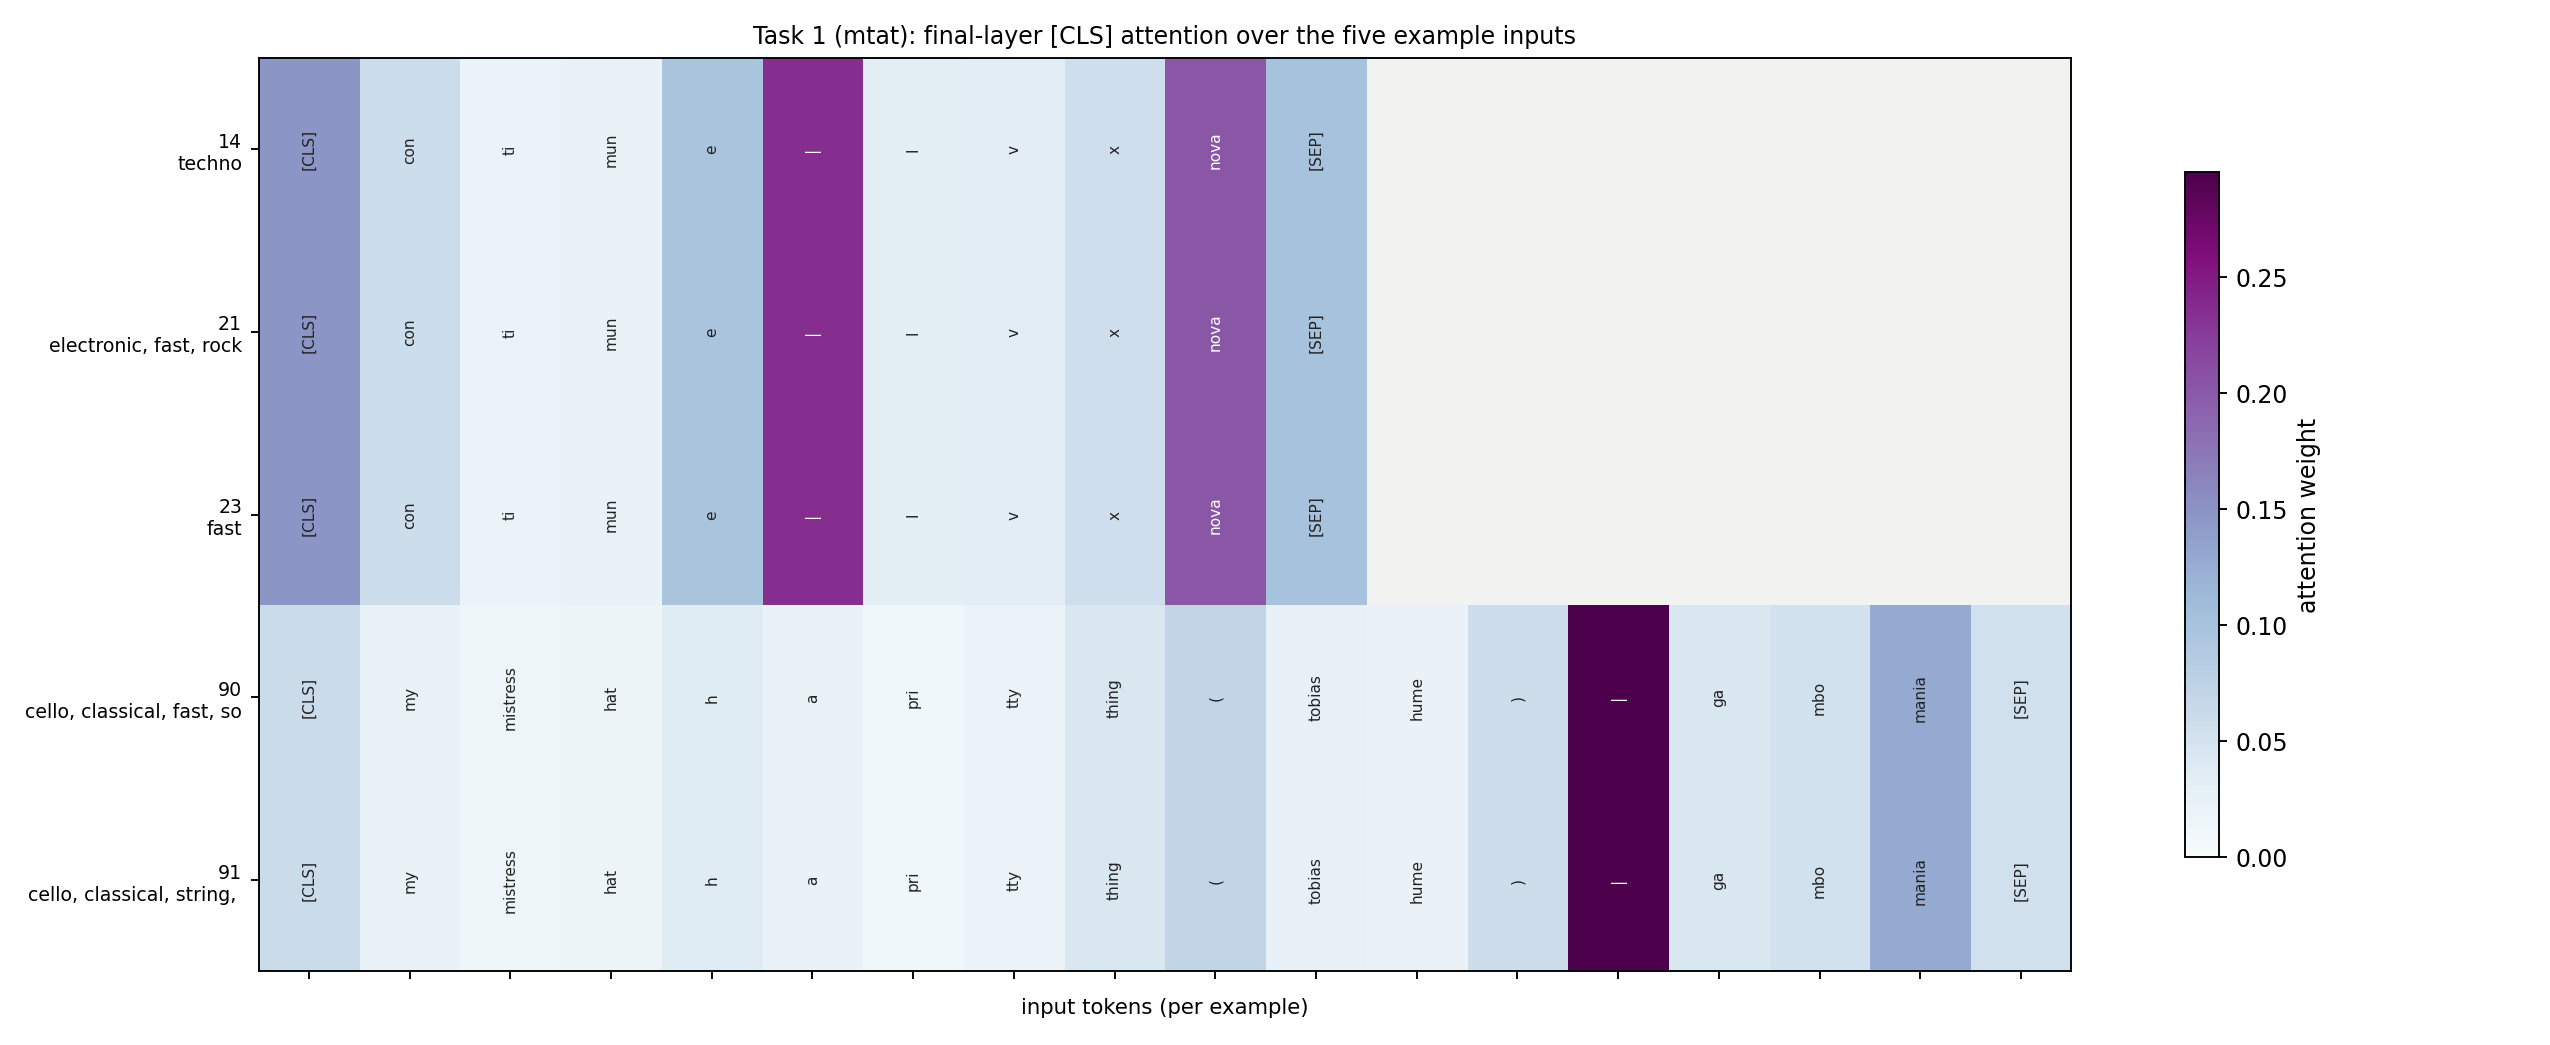
\includegraphics[width=\linewidth]{attention_task1_mtat.png}
\caption{Final-layer \texttt{[CLS]} attention, averaged over heads, for the five
committed MagnaTagATune example predictions --- the optional attention
visualisation named in the specification. It shows the duplicated-input ceiling
of Section~4.2 directly rather than as a statistic: clips $14$, $21$ and $23$
are three distinct clips whose text input is the same string
(\emph{Contimune $\mid$ LVX Nova}), so the attention pattern over them is
identical to five decimal places --- yet their ground-truth tags are
\emph{techno}, \emph{electronic/fast/rock} and \emph{fast} respectively. The
model cannot separate them because nothing in its input differs. Clips $90$ and
$91$ repeat the pattern. Mass concentrates on the separator and on the one
distinctive surname token rather than on any musical content word, which is what
a track-title corpus offers a language model to work with.}
\label{fig:attention}
\end{figure}

\begin{figure}[H]
\centering
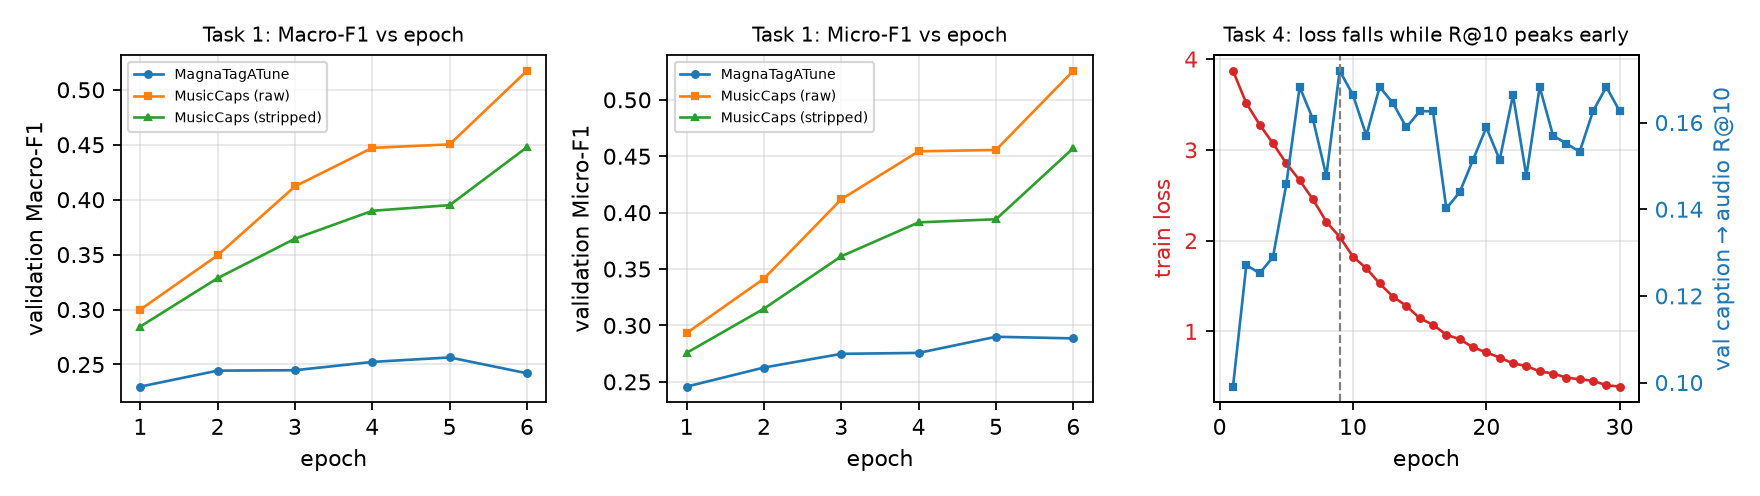
\includegraphics[width=\linewidth]{training_curves.png}
\caption{Validation Macro-F1 and Micro-F1 against training epoch for the three
Task 1 configurations (left, centre) --- the curve deliverable required by the
specification --- and Task 4's training dynamics (right). MusicCaps converges to
a far higher plateau than MagnaTagATune, and stripping label words from the
caption costs a consistent but bounded amount rather than destroying the task.
On the right, the InfoNCE loss falls monotonically from $3.87$ to $0.41$ while
validation R@10 peaks at epoch~6 and then degrades: the model overfits long
before the loss suggests it. The dashed line marks the epoch restored by
best-checkpoint selection.}
\label{fig:curves}
\end{figure}

\subsection{Task 2: structure graphs vs.\ a CNN}

\begin{table}[H]
\centering\small
\caption{Task 2. FMA-small genre classification, 8 balanced classes
(chance $=0.125$), artist-disjoint official splits.}
\setlength{\tabcolsep}{4pt}
\begin{tabular}{lccc}
\toprule
Model & Params & Acc. & Macro-F1 \\
\midrule
B4 PCA$+$MLP & 8,712 & 0.379 & 0.371 \\
GraphSAGE & 49,416 & 0.396 & 0.401 \\
GAT & \textbf{26,120} & 0.433 & 0.426 \\
CNN baseline (B2) & 241,992 & \textbf{0.483} & \textbf{0.479} \\
\bottomrule
\end{tabular}
\end{table}

\noindent All four sit well above the $0.125$ chance rate, and the ordering is
unambiguous: \textbf{the CNN wins on both metrics}, by $+0.050$ accuracy and
$+0.053$ Macro-F1 over the better graph model. GAT remains the most efficient
model, reaching $90\%$ of the CNN's accuracy with $9.3\times$ fewer parameters,
and both GNNs clear the B4 hand-crafted-feature baseline, so the graphs do
carry genre information. But the honest conclusion is stronger than in our
earlier draft: on FMA-small, relational structure is \emph{inferior to} --- not
merely competitive with --- treating the spectrogram as an image.

These numbers come from a cache rebuilt after the preprocessing crash described
in Section~\ref{sec:engineering}; the split (6{,}394/800/800, artist-disjoint,
verified zero leakage) is byte-identical to the earlier run, so the shifts are
attributable to the rebuilt features and not to a different partition.

\textbf{Which graph?} The specification names two structures, segment
similarity and chord transitions. Both are built by our pipeline, so we trained
the GNNs on each in turn --- identical splits, identical labels, identical
optimiser --- rather than assuming the choice.

\begin{table}[H]
\centering\small
\caption{Task 2, graph structure ablation. The same two encoders on the two
graph types the specification names, on identical artist-disjoint splits. The
CNN row is repeated for scale.}
\label{tab:graphtype}
\begin{tabular}{lcccc}
\toprule
& \multicolumn{2}{c}{Segment similarity} & \multicolumn{2}{c}{Chord transition} \\
\cmidrule(lr){2-3}\cmidrule(lr){4-5}
Model & Acc. & Macro-F1 & Acc. & Macro-F1 \\
\midrule
GraphSAGE & 0.396 & 0.401 & 0.339 & 0.316 \\
GAT & 0.433 & \textbf{0.426} & 0.303 & 0.271 \\
\midrule
CNN (B2) & \multicolumn{4}{c}{0.483 acc / \textbf{0.479} Macro-F1} \\
\bottomrule
\end{tabular}
\end{table}

\noindent The chord graph carries real signal --- $0.316$ Macro-F1 is
$2.5\times$ chance --- but it is clearly the weaker input, losing $0.110$
Macro-F1 to the segment graph and $0.163$ to the CNN. The reason is visible in
the graphs themselves: a $30$\,s clip collapses to roughly $21$ nodes drawn
from a $24$-triad vocabulary, and because each node's feature is that chord's
own pitch-class template, every trace of timbre, production and instrumentation
is discarded before the GNN sees anything. Genre on FMA-small is substantially
a timbral judgement, so the symbolic abstraction removes most of what the label
depends on. We report it because the negative result localises the problem: it
is the \emph{node features}, not message passing, that limit the chord graph.

\subsection{Are the graph's edges meaningful?}

The specification offers an optional diagnostic: the graph coherence score
$S_{\mathrm{graph}} = \frac{1}{|E|}\sum_{(i,j)\in E}\mathbb{1}[\cos(h_i,h_j) >
\tau]$, the fraction of edges whose endpoints the encoder maps to similar
representations. We report it as a sweep rather than a single number, because
node embeddings after ReLU are non-negative, so any low threshold marks
essentially every edge coherent whatever the graph contains --- at $\tau=0.5$
the score is $1.000$ for both a trained and an untrained encoder, and says
nothing.

\begin{table}[H]
\centering\small
\caption{Graph coherence over the 50 committed FMA sample graphs. ``Rewired''
draws the same number of edges at random between the same nodes; ``untrained''
is the same architecture at initialisation. A score is only meaningful against
these.}
\label{tab:coherence}
\begin{tabular}{lccc}
\toprule
$\tau$ & Real edges & Rewired & Untrained \\
\midrule
0.50 & 1.000 & 0.964 & 1.000 \\
0.80 & 0.982 & 0.840 & 0.994 \\
0.90 & 0.952 & 0.711 & 0.979 \\
0.95 & 0.870 & 0.546 & 0.944 \\
0.98 & 0.718 & 0.367 & 0.843 \\
0.99 & 0.560 & 0.261 & 0.722 \\
\bottomrule
\end{tabular}
\end{table}

\noindent The built edges separate clearly from rewired ones --- at $\tau=0.98$,
$0.718$ against $0.367$ --- so the wiring is not arbitrary. But the untrained
encoder scores $0.843$ on those same edges, \emph{higher} than the trained one,
and that is the informative part. Segment edges are created by thresholding
cosine similarity between node features in the first place, so their endpoints
begin similar and any encoder will map them to similar places. The coherence is
a property of how we built the graph, not something training discovered.
Training slightly reduces it, which is what an encoder learning to tell
adjacent segments apart should do.

This is a caution about the metric as much as about our graphs: reported alone
and at a permissive threshold, $S_{\mathrm{graph}}$ would have looked like
strong evidence that the graph structure was working, on a task where the
graph model loses to a CNN.

\subsection{Where the genre models succeed and fail}

\begin{table}[H]
\centering\small
\caption{Per-genre F1 on FMA-small. Both models rank the classes almost
identically, suggesting the difficulty is in the label taxonomy rather than the
architecture.}
\begin{tabular}{lcc}
\toprule
Genre & GAT & CNN (B2) \\
\midrule
Hip-Hop & 0.686 & 0.674 \\
Rock & 0.589 & 0.563 \\
Electronic & 0.509 & 0.537 \\
International & 0.493 & 0.600 \\
Instrumental & 0.374 & 0.466 \\
Folk & 0.304 & 0.292 \\
Pop & 0.281 & 0.368 \\
Experimental & 0.172 & 0.335 \\
\bottomrule
\end{tabular}
\end{table}

\noindent Hip-Hop is the easiest class for both models, and Experimental the
hardest for the GAT by a wide margin ($0.172$). This is informative:
``Experimental'' is a residual category defined by what it is not, so there is
no consistent acoustic signature to learn. The CNN's advantage is concentrated
in exactly the classes where the segment graph is least informative ---
Experimental ($+0.163$), Pop ($+0.087$) and International ($+0.107$) --- while
the GAT retains a small edge on the rhythmically distinctive Hip-Hop and Rock.
That pattern is consistent with the graph capturing coarse repetition structure
but discarding the timbral detail the spectrogram preserves.

\subsection{Task 3: fusion and its failure mode}
\label{sec:t3results}

\begin{table}[H]
\centering\small
\caption{Task 3 ablation. MagnaTagATune top-50, artist-grouped splits, zero
leakage. Every row is evaluated at the epoch chosen by best-validation
Macro-F1, never at a fixed final epoch. The last two rows are the two
follow-ups our earlier draft named as the experiments to try next.}
\label{tab:t3ablation}
\setlength{\tabcolsep}{4pt}
\begin{tabular}{lcccc}
\toprule
Mode & Params & Macro & Micro & AUC-PR \\
\midrule
BERT-only & 66.4M & 0.171 & 0.306 & 0.168 \\
GNN-only & 31.8K & 0.123 & 0.124 & 0.084 \\
Early concat & 66.4M & 0.168 & 0.314 & 0.182 \\
Cross-attention & 66.8M & 0.192 & 0.325 & 0.177 \\
\midrule
\quad $+$ frozen BERT & 0.5M & 0.118 & 0.315 & 0.197 \\
\quad $+$ non-BERT lr $10^{-3}$ & 66.8M & \textbf{0.246} & \textbf{0.415} & \textbf{0.248} \\
\bottomrule
\end{tabular}
\end{table}

\noindent \textbf{At a shared learning rate, fusion is marginal.} Cross-attention
gains $+0.022$ Macro-F1 and $+0.019$ Micro-F1 over BERT alone, but loses
$-0.005$ on AUC-PR to early concat. On their own these margins would be too
small to establish the project's central claim from a single seed.

\textbf{Why: the attention collapses completely.} Measuring the attention
distribution directly, the baseline cross-attention model has entropy
$\mathbf{1.000}$ of the uniform maximum with a peak-to-mean ratio of
$\mathbf{1.03\times}$ --- that is, the graph query does not discriminate
between caption tokens \emph{at all}, so $AH_{\mathrm{text}}$ degenerates to an
unweighted mean over the text and the model reduces to early concat. Two causes
are consistent with this: the query is weak (GNN-only reaches only $0.123$
Macro-F1 on 19-node graphs), and the text tower has $66.4$M parameters against
the graph branch's $31.8$K while sharing a single learning rate tuned for BERT
fine-tuning ($2\times10^{-5}$).

\textbf{The second cause is the operative one.} Raising the learning rate of
every parameter outside the text tower to $10^{-3}$ --- changing no
architecture, no data and no seed --- raises Macro-F1 from $0.192$ to
$\mathbf{0.246}$, Micro-F1 from $0.325$ to $\mathbf{0.415}$ and AUC-PR from
$0.177$ to $\mathbf{0.248}$. The same run's attention entropy falls from
$1.000$ to $0.695$ of uniform and its peak rises from $1.03\times$ to
$4.19\times$. The intervention that fixes the metric is the one that
demonstrably un-collapses the attention, which is the mechanism our diagnosis
predicted. Against BERT-only this is $+0.075$ Macro-F1 and $+0.109$ Micro-F1:
on this corpus, structural fusion helps once the non-BERT parameters are
actually trained. Which of them mattered --- the graph encoder, the
cross-attention block or the heads --- this experiment does not separate.

\noindent \textbf{What this does and does not isolate.} The parameter group is everything outside the text tower --- the graph encoder, the cross-attention block and both heads --- so the result establishes that a higher learning rate on the non-BERT parameters helps, not that the graph encoder specifically was the bottleneck. Separating those factors would need a per-module sweep we did not run. We name the effect after the optimiser change rather than after the module we suspect.

\textbf{The effect survives a seed sweep.} Because this is the report's central
positive claim, we re-ran both arms over five seeds (42, 1, 2, 3, 4) on one
machine. Since the two arms share seeds, the per-seed difference is paired and
we test it with a paired $t$-test.

\begin{table}[H]
\centering\small
\caption{Task 3 seed sweep, cross-attention, $n=5$ paired seeds. Mean $\pm$
sample standard deviation; $p$ from a two-sided paired $t$-test on the
per-seed difference.}
\label{tab:sweep}
\setlength{\tabcolsep}{3pt}
\begin{tabular}{lcccc}
\toprule
& Shared lr & Non-BERT lr & $\Delta$ & $p$ \\
\midrule
Macro-F1 & $.172\pm.023$ & $.240\pm.020$ & $+.067\pm.023$ & $.003$ \\
Micro-F1 & $.335\pm.024$ & $.416\pm.028$ & $+.081\pm.018$ & $.001$ \\
AUC-PR   & $.181\pm.015$ & $.260\pm.018$ & $+.079\pm.010$ & $<.001$ \\
\bottomrule
\end{tabular}
\end{table}

\noindent The difference is positive for \emph{every} seed (macro-F1 deltas
$+0.072, +0.040, +0.077, +0.098, +0.051$) and roughly three times the
seed-to-seed spread, so the gap is not an artifact of a lucky seed. We note
that seed-to-seed variation ($\pm0.023$ Macro-F1) exceeds several
between-ablation margins in Table~\ref{tab:t3ablation}, so those smaller
differences should not be read firmly. Seed 42 on different hardware gave
$0.254$, not $0.246$: the third decimal is not portable.

We state one further caveat plainly. The earlier draft's
conclusion that ``fusion does not clearly win'' was confounded by evaluating
every ablation at a fixed epoch~8 rather than at its best validation epoch ---
GNN-only, for instance, peaks at epoch~1 and has decayed to near-zero
validation Macro-F1 by epoch~8. Correcting the checkpoint policy changed the
ranking; it was a methodological error, not a discovery about fusion.

\textbf{Freezing BERT does not work.} The other follow-up --- freezing the text
tower so only the $0.5$M-parameter graph and fusion path train --- collapses
Macro-F1 to $0.118$ while producing the sharpest attention of any run (entropy
$0.079$, peak $10.02\times$) and, curiously, the second-best AUC-PR ($0.197$).
Sharp attention is therefore not sufficient: the model attends decisively to a
text representation it can no longer adapt.

\subsection{Task 3: the DEAM auxiliary term}

\begin{table}[H]
\centering\small
\caption{Effect of adding DEAM's valence/arousal term to cross-attention.
MagnaTagATune training data is identical across both columns, and both are
scored at their best validation epoch, the same policy used everywhere else in
this report.}
\label{tab:deam}
\begin{tabular}{lccc}
\toprule
Cross-attention & Tags only & $+$ DEAM & $\Delta$ \\
\midrule
Macro-F1 & 0.192 & 0.186 & $-0.007$ \\
Micro-F1 & 0.324 & 0.366 & $+0.041$ \\
AUC-PR & 0.176 & 0.212 & $+0.035$ \\
\midrule
Valence & --- & MAE 0.629 & $R^2\;+0.390$ \\
Arousal & --- & MAE 0.662 & $R^2\;+0.191$ \\
\bottomrule
\end{tabular}
\end{table}

\noindent The emotion heads work, and better than our first measurement
suggested: valence reaches $R^2 = 0.390$ and arousal $R^2 = 0.191$ on held-out
songs, so both beat predicting the training mean by a clear margin, with MAE of
$0.63$/$0.66$ on the normalised scale.

The more interesting correction is to the tag side. Our earlier draft reported
this run at a fixed final epoch and concluded that the auxiliary term costs
$36\%$ relative Macro-F1. Scored properly --- best validation checkpoint, as
in Table~\ref{tab:t3ablation} --- that penalty almost disappears: Macro-F1
falls by $0.007$, inside the $\pm0.023$ seed spread we measure in
Table~\ref{tab:sweep}, while Micro-F1 and AUC-PR both \emph{improve} by more
than $0.03$. The honest reading is that the multi-task term is roughly free on
this data rather than a trade-off, and that our earlier claim of a large penalty
was an artifact of the same checkpoint-policy error described below. We flag it
because the direction of the conclusion reversed, not merely its magnitude.

One reproducibility note. DEAM's official host (\texttt{cvml.unige.ch}) stopped
responding during this work and the audio mirror we located does not ship the
\texttt{metadata.zip} whose genre/artist/title fields build DEAM's
pseudo-captions; recovering that archive from a surviving mirror is what made
this re-run possible at all, and it is the single most fragile external
dependency in the project.

\subsection{Task 4: cross-modal retrieval}

\begin{table}[H]
\centering\small
\caption{Task 4. MusicCaps retrieval on the \emph{official} AudioSet eval
partition: a gallery of 2{,}773 clips, $5.2\times$ larger than the random-split
gallery of 536 we reported earlier. R@K falls sharply with gallery size, so the
two are not comparable in absolute terms and we give the random baseline for
scale. ``Separate graph lr'' applies the Task 3 finding to this task.}
\label{tab:retrieval}
\begin{tabular}{llccc}
\toprule
Run & Direction & R@1 & R@5 & R@10 \\
\midrule
Shared lr & Caption $\to$ Audio & 0.0029 & 0.0108 & 0.0220 \\
          & Audio $\to$ Caption & 0.0022 & 0.0126 & 0.0224 \\
\midrule
Separate  & Caption $\to$ Audio & \textbf{0.0058} & \textbf{0.0173} & \textbf{0.0339} \\
graph lr  & Audio $\to$ Caption & 0.0054 & 0.0184 & 0.0317 \\
\midrule
Random    & ---                 & 0.0004 & --- & 0.0036 \\
\bottomrule
\end{tabular}
\end{table}

\noindent \textbf{The Task 3 finding transfers.} Giving the non-BERT parameters their own
learning rate of $10^{-3}$ --- the intervention that un-collapsed the fusion
attention in Section~\ref{sec:t3results}, here tested rather than assumed to
carry over --- doubles R@1 and lifts R@10 from $0.0220$ to $0.0339$, or
$9.4\times$ random. Median rank improves from $527$ to $400$ of $2{,}773$. That
the same single hyperparameter governs both a supervised fusion model and a
contrastive dual encoder is the strongest evidence we have that the graph
branch, not the architecture, was the binding constraint throughout this
project.

The absolute numbers nevertheless stay low, and we wanted to know whether that
is a modelling failure or a data-budget one. Holding the validation set, test
set and gallery fixed and subsampling only the training pairs gives a clean
answer.

\begin{table}[H]
\centering\small
\caption{Task 4 retrieval against training-set size. Only the training split is
subsampled; validation, test and the 2{,}773-clip gallery are held fixed, so
R@K is comparable down the column. Single seed per point.}
\label{tab:scale}
\begin{tabular}{lccc}
\toprule
Train pairs & C$\to$A R@10 & A$\to$C R@10 & vs.\ random \\
\midrule
549   & 0.0155 & 0.0162 & $4.3\times$ \\
1,098 & 0.0206 & 0.0216 & $5.7\times$ \\
1,646 & 0.0325 & 0.0274 & $9.0\times$ \\
2,195 & \textbf{0.0339} & 0.0317 & $\mathbf{9.4\times}$ \\
\bottomrule
\end{tabular}
\end{table}

\noindent R@10 grows log-linearly in the number of paired examples
($R^2 = 0.914$, $+0.0099$ R@10 per doubling; Figure~\ref{fig:scale}) with no
convincing sign of saturation --- the last interval flattens, but by less than
single-seed noise. Extrapolating the fit, reaching a usable R@10 of $0.10$ would
need on the order of $2\times10^5$ paired clips, roughly $100\times$ what the
official split provides. That figure characterises a regime; it is not a
forecast, and we would not defend it as one. It rests on four single-seed
points spanning less than one order of magnitude, extrapolated across two,
and it assumes the log-linear trend continues rather than saturating --- which the last interval may already be doing, by less than single-seed
noise. The defensible claim is the direction and the orderliness of the
trend, not the number of clips.

The conclusion we draw is specific. Our contrastive result is weak, but it is
weak in the way a data-starved model is weak rather than a broken one --- the
scaling behaviour is orderly, the direction is right, and every doubling buys a
predictable amount. MusicCaps at $5{,}521$ clips is simply a small corpus for
contrastive alignment, and the official partition spends half of it on
evaluation.

\begin{figure}[H]
\centering
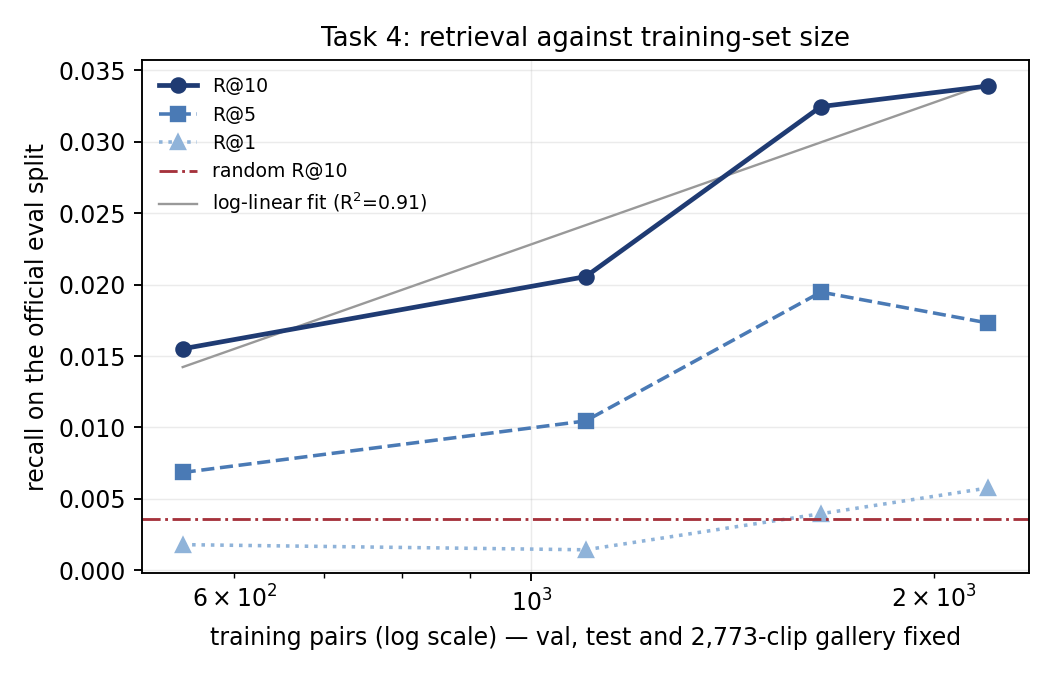
\includegraphics[width=\linewidth]{task4_scale.png}
\caption{Task 4 R@10 against training-set size on a log axis, gallery held
fixed at 2{,}773 clips. The fit is log-linear ($R^2 = 0.914$); the dashed
horizontal line is the random baseline.}
\label{fig:scale}
\end{figure}

\textbf{Zero-shot tagging, against the supervised model on identical data.}
The specification asks for zero-shot tagging measured against the Task~3
supervised model. Both models therefore derive their split from one shared
function (\texttt{src/splits.official\_eval\_split}) and their vocabulary from
the training clips of that split, and each writes its test clip ids and its
vocabulary into its own metrics file so the equality can be \emph{checked}
rather than assumed: the two runs score the same $2{,}773$ clips against the
same $50$ tags.

\begin{table}[H]
\centering\small
\caption{Zero-shot versus supervised on verified-identical data: same corpus,
same official eval clips, same 50 tags derived from training clips only.
Neither the zero-shot vocabulary nor its threshold sees a test label.}
\label{tab:zeroshot}
\begin{tabular}{lccc}
\toprule
& Micro-F1 & Macro-F1 & AUC-PR \\
\midrule
Task 3, supervised fusion & \textbf{0.657} & \textbf{0.588} & \textbf{0.624} \\
Task 4, zero-shot & 0.098 & 0.096 & 0.059 \\
\bottomrule
\end{tabular}
\end{table}

\noindent Contrastive alignment alone recovers about $15\%$ of supervised
Micro-F1. Two corrections sit behind that number and we record both. Our first
draft compared against Task~1 rather than Task~3, and its zero-shot protocol
leaked: the vocabulary was chosen by frequency \emph{in the test split} and the
threshold tuned on test labels. The encoder never saw tag supervision, but the
evaluation read the answers twice. A second, subtler version of the same fault
survived the first fix --- the two scripts derived the split independently, one
shuffling the pool and one not, so equal split \emph{sizes} concealed different
train/validation membership while nothing printed disagreed. Sharing one split
function and logging the clip ids is what makes the comparison checkable.

\subsection{Task 4: what listeners said}

The specification asks for a human study on Task 4. Six listeners rated each of
the thirty retrieved clips from 1 (unrelated) to 5 (matches closely), against
the caption that retrieved it.

\begin{table}[H]
\centering\small
\caption{Task 4 human evaluation. Six listeners, $174$ ratings, $1$--$5$ for
whether the retrieved clip matches its query caption. Clip order was randomised
per listener so the model's ranking was not visible to them.}
\label{tab:human}
\begin{tabular}{lccc}
\toprule
& Mean & SD & $n$ \\
\midrule
All ratings & $1.79$ & $1.36$ & 174 \\
\midrule
Rank 1 & $2.03$ & $1.51$ & 60 \\
Rank 2 & $1.28$ & $0.69$ & 60 \\
Rank 3 & $2.07$ & $1.59$ & 54 \\
\bottomrule
\end{tabular}
\end{table}

\noindent \textbf{Listeners agree with R@K.} A mean of $1.79$ on a five-point
scale says most retrieved clips do not match the caption that retrieved them.
That is what Table~\ref{tab:retrieval} already implied --- with R@10 at
$0.0339$ and a median true-clip rank of $400$, the three clips a listener sees
usually do not contain the right one. Two independent instruments, one
automatic and one human, place this system in the same place, which is stronger
evidence than either alone.

\textbf{The model's own ranking carries no signal for listeners.} Rank~2 scores
\emph{below} both rank~1 and rank~3, and the correlation between a clip's
similarity score and its mean human rating is $r = -0.051$ --- indistinguishable
from none. So within the top three the ordering is arbitrary to a listener, even
though those three were selected out of a $2{,}773$-clip gallery. This is
consistent with the picture in Section~\ref{sec:t3results}: the learned space
separates relevant from irrelevant weakly, and does not rank finely within what
it has already selected.

\textbf{Retrieval is more often plausible than correct.} Fourteen of the $174$
ratings were $4$ or $5$, spread across most queries, while only $0.58\%$ of
queries place the true clip at rank~1. A clip can legitimately match a generic
caption without being the annotated one, so the human study measures something
R@K cannot: the model finds \emph{believable} audio considerably more often than
it finds the \emph{intended} audio. For a retrieval system that distinction
matters, and it is invisible to recall alone.

\textbf{Study design.} Each listener saw one clip per screen with its caption,
and the three clips for a caption were presented in a random order, so the
ranking under test was never visible. A clip that could not be played was
recorded as a gap rather than a low score: one clip was unavailable and all six
listeners marked it so, giving $174$ ratings rather than $180$. Time on task
ranged from $6.3$ to $17.3$ minutes against $5.0$ minutes of audio, so no
submission was faster than listening allows.

\subsection{Qualitative analysis of the fused space}

\begin{figure}[H]
\centering
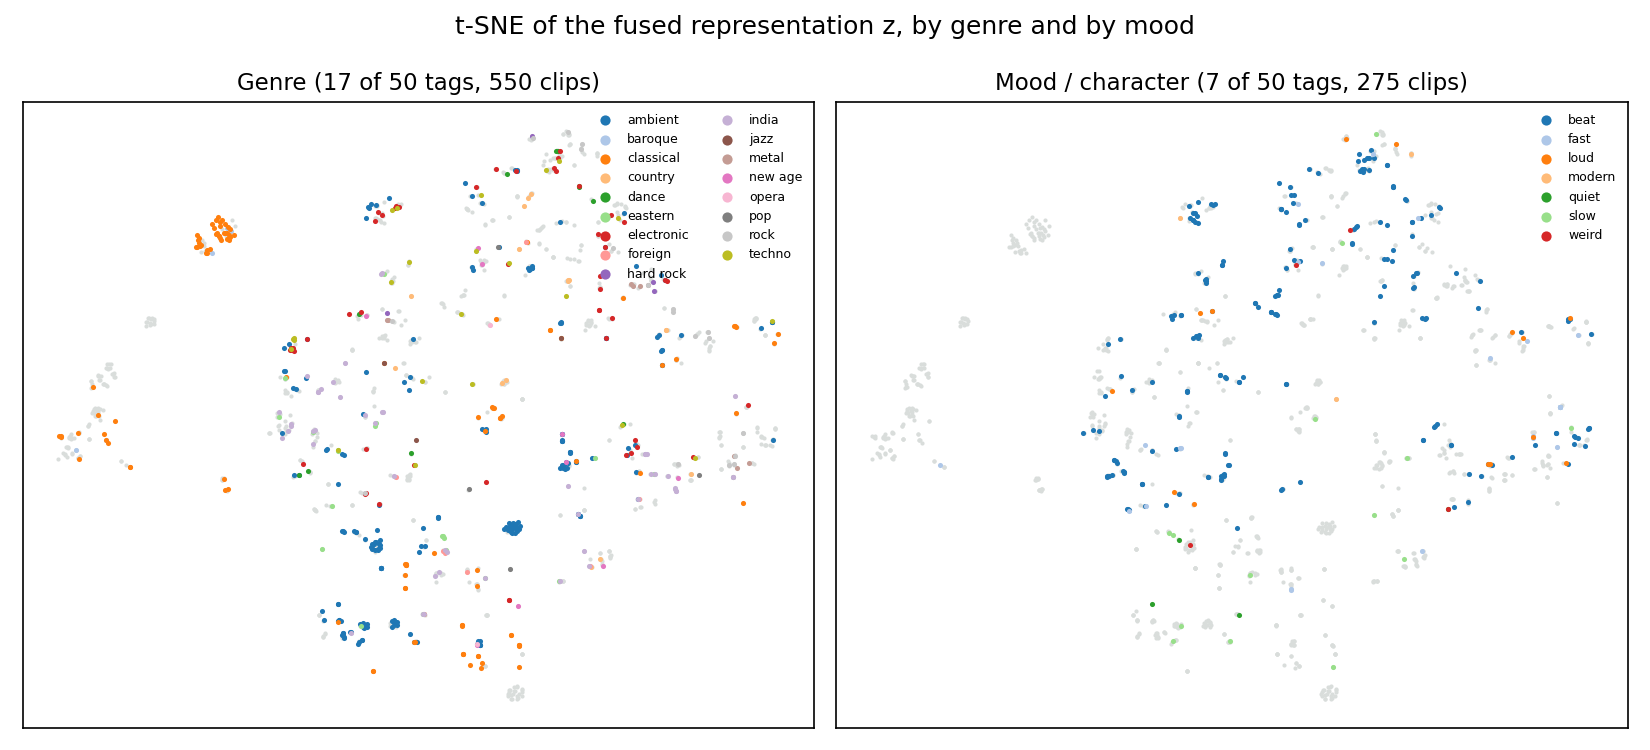
\includegraphics[width=\linewidth]{tsne_task3_views.png}
\caption{t-SNE of the fused representation $z$ (cross-attention, $384$-dim)
over $1{,}500$ held-out MagnaTagATune clips, split into the two views the
specification asks for. Each clip is coloured by its \emph{primary} tag --- the
single highest-prevalence tag it carries --- not by its full multi-label
annotation, and clips whose primary tag falls outside the panel's vocabulary are
drawn in grey. MagnaTagATune's top-50 list mixes genre, mood, instrument and
production descriptors in one flat vocabulary, so the split is ours: the mood
panel is a proxy that includes tempo and production words (\emph{fast},
\emph{quiet}, \emph{loud}) alongside affective ones. Broad timbral families
separate --- classical and vocal-led material occupy distinct regions --- but
the structure is diffuse rather than cleanly clustered, consistent with the
modest Macro-F1 in Table~\ref{tab:t3ablation}.}
\end{figure}

\noindent \textbf{Case studies.} Table~\ref{tab:cases} pairs graph structure
with the caption tokens the graph vector attends to, for three held-out clips
from distinct tracks.

\begin{table}[H]
\centering\scriptsize
\caption{Three case studies. ``Attn.\ spread'' is the ratio of largest to
smallest attention weight over the top-8 tokens; values near $1.0$ indicate
the collapse discussed in Section 5.3.}
\label{tab:cases}
\begin{tabular}{p{0.30\linewidth}p{0.30\linewidth}c}
\toprule
True tags & Top predictions & Attn.\ spread \\
\midrule
drum, electronic, synth, weird & techno, electronic, beat & 1.03 \\
ambient, flute, new age & drum, india, ambient & 1.03 \\
beat, electronic, fast, techno & rock, male vocal, vocal & 1.11 \\
\bottomrule
\end{tabular}
\end{table}

\noindent The first case is a partial success: an electronic track tagged
\emph{drum, electronic, synth} is predicted \emph{techno, electronic, beat},
capturing the family if not the exact vocabulary. The third is a clear failure:
an electronic/techno clip is predicted \emph{rock, male vocal, guitar}. In every
case the attention spread is within $3\%$ of uniform, so these predictions are
driven by the text mean and the graph vector, not by any selective reading of
the caption. These case studies come from the shared-learning-rate model; the
separate-learning-rate run does attend selectively (peak $4.19\times$ uniform).

\subsection{A control: the same fusion on text that describes the audio}

Our central Task 3 claim is that the cross-attention collapses because
MagnaTagATune's text is track-level metadata with nothing to attend to, not
because the architecture is wrong. That is testable, so we tested it: the
identical model, hyperparameters and separate graph learning rate, trained on
MusicCaps graphs and captions over the 50 aspects Task 1 uses
($3{,}748/803/804$ split).

\begin{table}[H]
\centering\small
\caption{The same architecture on two corpora. The F1 rows are \emph{not} a
like-for-like comparison --- different corpus, labels and difficulty --- and are
given only so the attention rows, which are comparable, can be read in context.}
\label{tab:textcontrol}
\begin{tabular}{lcc}
\toprule
& MagnaTagATune & MusicCaps \\
& (metadata) & (descriptions) \\
\midrule
Macro-F1 / Micro-F1 & 0.246 / 0.415 & 0.673 / 0.727 \\
Attention entropy & 0.695 & \textbf{0.393} \\
Peak over uniform & $4.19\times$ & $\mathbf{29.4\times}$ \\
Case-study spread & $1.03$--$1.11\times$ & $3.6$--$58.5\times$ \\
\bottomrule
\end{tabular}
\end{table}

\noindent \textbf{The collapse is a property of the text, not the
architecture.} Given real captions the same cross-attention becomes sharply
selective --- entropy $0.393$ of uniform, peaks near $30\times$ --- where on
MagnaTagATune its case-study weights sat within $3\%$ of uniform. That is the
control the diagnosis needed.

\textbf{The F1 gap is not a win, and we do not report it as one.} MusicCaps
aspects appear verbatim in their own captions; Section~\ref{sec:t1results}
measures a lexical-match baseline at Micro-F1 $0.540$ on this exact material, so
a model reading them is partly doing substring detection. The attention
statistics are the result here, not the accuracy.

The case studies are correspondingly richer than Table~\ref{tab:cases}'s, which
could only align a graph against a track title: a caption describing
``digital drums \dots\ two guitars \dots\ an e-bass \dots\ a piano'' draws
\emph{piano} and \emph{e-bass} into the top four, and each of the three cases
recovers two true aspects. One caveat is visible in the weights themselves --
the highest-attention tokens are determiners and copulas (\emph{this},
\emph{is}, \emph{the}), not the musical content words. The attention is sharp
without being semantic, which is the freeze-BERT lesson of
Section~\ref{sec:t3results} arriving from the opposite direction: sharpness is
necessary for the mechanism to be doing anything, and is not evidence that it
is doing the right thing.

\noindent \textbf{Graph paths.} Each case study records a walk through its
segment graph, so a route can be read against the caption: it starts at the
highest-degree segment and steps to unvisited neighbours. Segment $k$ covers
seconds $1.5k$--$1.5(k{+}1)$, so the walk $[1,0]$ names $1.5$--$3.0$\,s then
$0$--$1.5$\,s. It is an illustrative walk and nothing more: it is unweighted,
because the edge weights the cache stores were not carried into the graphs these
case studies came from, and its stopping after two nodes says only that the
greedy walk ran out of unvisited neighbours --- not that the graph lacks longer
paths, which would need a path statistic we did not compute.

\noindent \textbf{Retrieval behaviour.} Across the official-split gallery of
$2{,}773$ clips the median true-clip rank is $527$, placing the correct clip in
the top $19\%$ of the gallery on average --- clearly better than chance
($8.0\times$ random at R@1), but far from usable retrieval. The
model appears to learn coarse acoustic-descriptive correspondence (recording
quality, instrumentation family, tempo band) without the fine discrimination
that rank-1 retrieval demands.

\section{Engineering Findings}
\label{sec:engineering}
Several results in this report depended on catching pipeline defects that
produce plausible-looking numbers. We record them because each was silent.

\textbf{Near-complete graphs.} Our first graph build produced $19.4$-node
graphs with average degree $18.15$ --- effectively complete. A GNN over a
complete graph computes the same neighbourhood for every node, so message
passing reduces to global mean pooling and the architecture becomes
irrelevant while still training and reporting sensible-looking accuracy. The
cause was that raw MFCC descriptors share a large positive mean, giving median
pairwise cosine similarity $0.9971$. Only after z-scoring within each track did
the threshold behave as intended.

\textbf{The opposite failure.} Having fixed the scaling, the threshold constant
was left at its old value, producing average degree $1.90$ --- a bare temporal
chain with \emph{zero} similarity edges. Both failures produce trainable models;
neither announces itself.

\textbf{A silent truncated cache.} Serialising the preprocessed
MagnaTagATune cache wrote a zero-byte file without raising, because the
log-mel component alone was $3.49$\,GB of a $3.6$\,GB structure. Since only the
CNN baseline consumes log-mel, it is now optional.

\textbf{Threshold selection.} Multi-label probabilities under
prevalence-weighted BCE do not centre at $0.5$; our tuned thresholds ranged from
$0.7$ to $0.8$. Evaluating at $0.5$ would have understated every Task 1 and
Task 3 result substantially.

\textbf{A segfault that looked like a deadlock.} The graph builder appeared to
hang: it froze at $4{,}000/8{,}000$ FMA tracks and, on another run, at
$10{,}500/21{,}318$ MagnaTagATune clips, with every worker asleep on a futex at
$\approx0$\,s of CPU. The real event was a \emph{segmentation fault} inside a
numba \texttt{guvectorize} kernel reached through
\texttt{librosa}~\cite{librosa} \texttt{chroma\_stft} $\to$ \texttt{estimate\_tuning} $\to$
\texttt{piptrack}, caused by a \texttt{numba} $0.67$ / \texttt{numpy} $2.1$ ABI
mismatch in the GPU image. The deadlock appearance is a property of
\texttt{multiprocessing.Pool}: it silently respawns a worker that dies mid-task
and simply never delivers that task's result, so the parent blocks forever.
Pinning the numba/llvmlite pairing fixed the crash, and replacing the pool with
\texttt{ProcessPoolExecutor} --- which raises \texttt{BrokenProcessPool}
immediately on worker death --- converted an hour of silent stalling into an
instant diagnosable failure. Throughput also rose from $8.8$ to $16.2$
tracks/s.

\textbf{Two split defects.} Our Task 1 and Task 4 MusicCaps experiments
originally used random splits even though the metadata ships an
\texttt{is\_audioset\_eval} flag defining the official partition; the corrected
official-split results are materially worse and are what this report now
carries. Separately, the Task 1 random baseline estimated per-tag prevalence
from \emph{test} labels, which leaks test statistics into a baseline; it now
uses training labels only.

\textbf{Checkpoint policy.} Task 1 and Task 3 evaluated whichever epoch
happened to be last rather than restoring the best validation checkpoint. This
was not cosmetic: Task 3's GNN-only ablation peaks at epoch~1 and decays to
near-zero validation Macro-F1 by epoch~8, and correcting it changed the ranking
of the Task 3 ablation table.

We mention these not as incidental debugging notes but because most of them
would have yielded a complete, publishable-looking results table built on a
model, a split, or a baseline that was not doing what its description claimed.

\section{Discussion and Limitations}

Three limitations bound what these results can claim.

\textbf{The text is impoverished.} For MagnaTagATune our BERT branch sees only
``title $\mid$ album''. This is the source of both the $0.673$ ceiling and,
plausibly, the attention collapse: there is little in a track title for a graph
vector to select between. A corpus pairing audio with genuine descriptive text
at clip granularity --- as MusicCaps does --- is the right setting for fusion,
and our Task 1 results support this, with stripped-caption Micro-F1 of
$0.488$ versus $0.275$.

\textbf{The graph branch was under-trained, and fixing that was decisive.}
GNN-only reaches $0.123$ Macro-F1 with $31.8$K parameters against BERT's
$66.4$M, sharing one learning rate. We ran both diagnostics this predicted. A
separate graph-branch learning rate of $10^{-3}$ raised cross-attention
Macro-F1 from $0.192$ to $0.246$ and Micro-F1 from $0.325$ to $0.415$ while
cutting attention entropy from $1.000$ to $0.695$ of uniform; freezing BERT
instead produced the sharpest attention of any run but the worst Macro-F1. The
conclusion is that the shared learning rate, not the architecture, was the
binding constraint --- and that attention sharpness alone is not a sufficient
indicator of a working fusion. A five-seed paired sweep confirms the effect
($+0.067 \pm 0.023$ Macro-F1, $p = 0.003$, positive on every seed). The natural
next step is to tune the graph-branch learning rate properly rather than
accepting the first value we tried.

\textbf{Segment graphs may be the wrong structure, and the alternative is
worse.} Our nodes are fixed $1.5$\,s windows. Table~\ref{tab:graphtype} shows
the chord-transition graph the specification also names performs $0.110$
Macro-F1 below it, so the segment graph is the better of the two structures we
built --- but a $19$-node graph over uniform windows may still encode little
beyond a smoothed timeline, and beat-synchronous segmentation, which we
implement but did not train on, remains untested. The chord result suggests the
limitation is in the node features rather than in message passing.

\textbf{The human study is small, and its scale is its limit.} Six listeners
and $174$ ratings is enough to establish that retrieved clips mostly do not
match their captions, and enough to show that the model's ranking does not
predict human judgement. It is not enough to estimate either quantity
precisely, to model listener effects, or to detect a small difference between
ranks. Listeners were not screened for musical training or hearing, and with
six raters no such split would have been interpretable. We therefore report the
aggregate and the per-rank means, and make no claim resting on a difference
smaller than the spread between listeners, whose means range from $1.28$ to
$2.48$.

\textbf{Single seeds.} Every result in this report except the Task 3
learning-rate comparison and the Task 1 curves comes from one seed. Our own
sweep puts seed-to-seed spread at $\pm0.023$ Macro-F1, which exceeds several of
the margins in Table~\ref{tab:t3ablation}; those rankings should be read as
indicative. The data-scale points in Table~\ref{tab:scale} are likewise single
seed, which is why we treat the flattening in the last interval as noise rather
than saturation.

\section{Conclusion}
We implemented all four tasks. Our first conclusion about fusion was negative
and turned out to be an optimisation artefact: under a single learning rate the
cross-attention collapses and fusion loses, and once the non-BERT parameters
train at their own rate the same architecture beats its text branch. We regard
the diagnosis, and the correction of our own claim, as the contribution: a measured
performance ceiling from duplicated inputs, a measured artist leak in a
standard split, a measured attention collapse, a multi-task term that proved
roughly free rather than costly once our own checkpoint policy was corrected,
and a human study that agrees with the automatic metric while showing the
ranking beneath it to be arbitrary. Each of these would have been invisible had we reported only
headline F1 against no baseline --- and in one case (raw-caption tagging) doing
so would have overstated our result roughly fivefold. Cross-modal fusion for
music context understanding remains plausible; this work delimits the
conditions under which it can be demonstrated.

\section*{Reproducibility}
Code, seeded configurations, per-run metrics, $155$ example graphs
($50$ FMA, $105$ MagnaTagATune, each as both \texttt{.pt} and \texttt{.json}
with an index manifest), the t-SNE projection and all training logs are in the
project repository. Every number in this report is lifted from
\texttt{results/metrics.json} into \texttt{report/\_numbers.json} by
\texttt{src/aggregate\_metrics.py} and \texttt{src/make\_report\_numbers.py},
so the paper's reference values cannot be older than the runs they describe.
The train/validation/test manifests for all three corpora are committed under
\texttt{data/splits/}, so the exact partition behind every number can be
inspected without re-running preprocessing.
Training requires a GPU; every evaluation, plot and notebook in the repository
runs on CPU in seconds from the committed artifacts. The human study ran as a
web application whose source, stimuli and per-listener submissions are all
committed, so it can be repeated with new listeners rather than merely
described. The Task 1 MusicCaps checkpoint is downloadable with a published
SHA-256; the download, checksum check and a single inference call were verified
from a clean copy, and \texttt{artifacts/checkpoints/README.md} carries the
commands.

\begin{thebibliography}{10}\footnotesize\setlength{\itemsep}{0pt}\setlength{\parskip}{0pt}
\bibitem{fma} M. Defferrard et al., ``FMA: A Dataset For Music Analysis,''
\emph{ISMIR}, 2017.
\bibitem{mtat} E. Law et al., ``Evaluation of Algorithms Using Games: The Case
of Music Tagging,'' \emph{ISMIR}, 2009.
\bibitem{deam} A. Aljanaki, Y.-H. Yang and M. Soleymani, ``Developing a
Benchmark for Emotional Analysis of Music,'' \emph{PLoS ONE}, 2017.
\bibitem{musiccaps} A. Agostinelli et al., ``MusicLM: Generating Music From
Text,'' \emph{arXiv:2301.11325}, 2023.
\bibitem{sage} W. Hamilton, Z. Ying and J. Leskovec, ``Inductive
Representation Learning on Large Graphs,'' \emph{NeurIPS}, 2017.
\bibitem{gat} P. Veli\v{c}kovi\'{c} et al., ``Graph Attention Networks,''
\emph{ICLR}, 2018.
\bibitem{bert} J. Devlin et al., ``BERT: Pre-training of Deep Bidirectional
Transformers for Language Understanding,'' \emph{NAACL}, 2019.
\bibitem{distilbert} V. Sanh et al., ``DistilBERT, a distilled version of
BERT,'' \emph{arXiv:1910.01108}, 2019.
\bibitem{infonce} A. van den Oord, Y. Li and O. Vinyals, ``Representation
Learning with Contrastive Predictive Coding,'' \emph{arXiv:1807.03748}, 2018.
\bibitem{librosa} B. McFee et al., ``librosa: Audio and Music Signal Analysis
in Python,'' \emph{SciPy}, 2015.
\end{thebibliography}

\end{document}
